% Vector artwork: scientific workflow, with construction/evaluation boundary.
\begingroup%
\definecolor{flowink}{HTML}{17324D}%
\definecolor{flowteal}{HTML}{167D8D}%
\definecolor{flowblue}{HTML}{EEF4F8}%
\definecolor{flowgold}{HTML}{B36B25}%
\resizebox{\linewidth}{!}{%
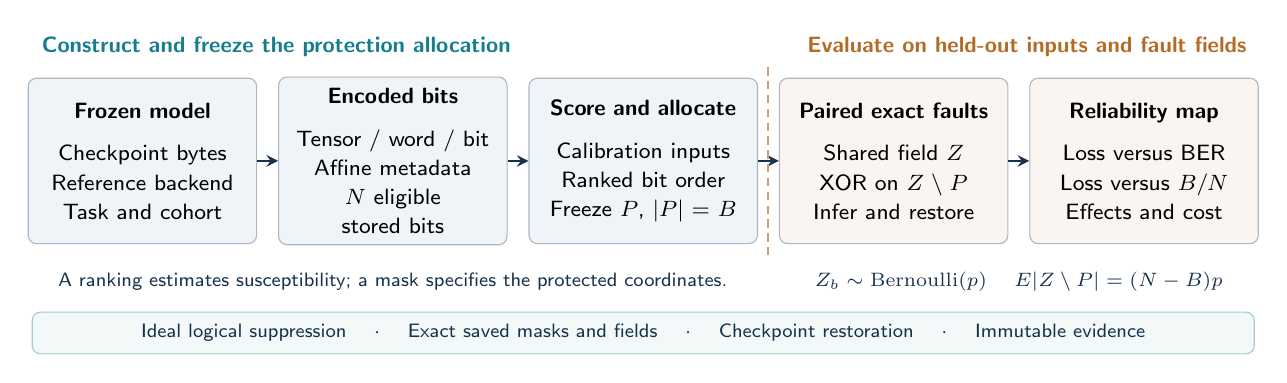
\begin{tikzpicture}[font=\sffamily\fontsize{8.5}{10.5}\selectfont,>=stealth,
  stage/.style={draw=flowink!35,fill=flowblue,rounded corners=3pt,
    minimum width=2.80cm,minimum height=2.10cm,text width=2.62cm,align=center,
    inner sep=4pt},
  edge/.style={->,draw=flowink,line width=0.85pt}]
\node[anchor=west,font=\sffamily\bfseries\footnotesize,text=flowteal] at (-1.4,1.45)
  {Construct and freeze the protection allocation};
\node[anchor=west,font=\sffamily\bfseries\footnotesize,text=flowgold] at (8.32,1.45)
  {Evaluate on held-out inputs and fault fields};
\node[stage] (model) at (0,0)
  {\textbf{Frozen model}\\[5pt]Checkpoint bytes\\Reference backend\\Task and cohort};
\node[stage] (bits) at (3.18,0)
  {\textbf{Encoded bits}\\[5pt]Tensor / word / bit\\Affine metadata\\$N$ eligible stored bits};
\node[stage] (mask) at (6.36,0)
  {\textbf{Score and allocate}\\[5pt]Calibration inputs\\Ranked bit order\\Freeze $P$, $|P|=B$};
\node[stage,fill=flowgold!7] (fault) at (9.54,0)
  {\textbf{Paired exact faults}\\[5pt]Shared field $Z$\\XOR on $Z\setminus P$\\Infer and restore};
\node[stage,fill=flowgold!7] (result) at (12.72,0)
  {\textbf{Reliability map}\\[5pt]Loss versus BER\\Loss versus $B/N$\\Effects and cost};
\draw[edge] (model)--(bits);
\draw[edge] (bits)--(mask);
\draw[edge] (mask)--(fault);
\draw[edge] (fault)--(result);
\draw[flowgold!65,densely dashed,line width=0.7pt] (7.95,-1.20)--(7.95,1.26);
\node[align=center,text=flowink,font=\sffamily\scriptsize] at (3.18,-1.53)
  {A ranking estimates susceptibility; a mask specifies the protected coordinates.};
\node[align=center,text=flowink,font=\sffamily\scriptsize] at (11.13,-1.53)
  {$Z_b\sim\mathrm{Bernoulli}(p)$ \quad $\mathbb{E}|Z\setminus P|=(N-B)p$};
\draw[draw=flowteal!40,fill=flowteal!5,rounded corners=3pt]
  (-1.40,-2.45) rectangle (14.12,-1.92);
\node[text=flowink,font=\sffamily\scriptsize] at (6.36,-2.185)
  {Ideal logical suppression \quad $\cdot$ \quad Exact saved masks and fields \quad $\cdot$ \quad Checkpoint restoration \quad $\cdot$ \quad Immutable evidence};
\end{tikzpicture}%
}%
\endgroup%
